\section{Quick start: run the whole pipeline}
\label{sec:quick}

\subsection{Purpose and plan}

The quick start exercises every part of the pipeline that does not need the board, in an order
chosen so that each step tests one new thing (Table~\ref{tab:quick}). A failure therefore points
at one component. All commands are run in a PowerShell window in which the opening sequence of
Section~\ref{sec:opening} has been given, so that the prompt reads
\venvprompt

\begin{table}[H]
\centering
\begin{tabular}{C{0.9cm}L{4.3cm}L{3.9cm}C{1.7cm}}
\toprule
\hd{Step} & \multicolumn{1}{c}{\hd{Action}} & \multicolumn{1}{c}{\hd{What it tests}} & \hd{Time} \\
\midrule
\ref{st:pytest} & Run the automatic tests & The code and the Python packages & 1 min \\
\ref{st:render} & Make 80 simulated photographs & MiKTeX and Poppler & 2--5 min \\
\ref{st:synth} & Generate training images & Fonts and image processing & 2--3 min \\
\ref{st:train} & Train the classifier & TensorFlow & 45--75 min \\
\ref{st:eval} & Measure accuracy on the 80 photographs & The complete pipeline & 3 min \\
\ref{st:review} & Produce the review document & Photographs beside results & 2 min \\
\ref{st:onephoto} & Turn one photograph into a PDF & The application and its output & 1 min \\
\bottomrule
\end{tabular}
\caption{The steps of the quick start.}
\label{tab:quick}
\end{table}

\subsection{The automatic tests}

\step{Make sure the window is ready}\label{st:quickready}
% The opening sequence, written out in full. Input wherever a session may begin in a new window.
Look at the prompt of the PowerShell window. If it begins with \texttt{(.venv)} and shows the
project folder, go on to the next step. If the window is new, or its prompt lacks
\texttt{(.venv)} or shows another folder, give the two commands of the opening sequence.
\begin{ps}[Opening sequence, command 1 of 2]
cd C:\ee105\camera-to-latex
\end{ps}
\begin{ps}[Opening sequence, command 2 of 2]
.\.venv\Scripts\Activate.ps1
\end{ps}
\checkpoint{The prompt reads:}
\venvprompt


\step{Run the tests}\label{st:pytest}
\begin{ps}
python -m pytest -q
\end{ps}
The project contains small programs that check its own code: for example, that a symbol drawn
above the line is read as a superscript, and that a frame with a wrong checksum is rejected.
Each dot in the output is one test that passed.
\begin{out}
................................................                         [100%]
48 passed in 9.87s
\end{out}
\checkpoint{The last line says \emph{48 passed} and does not contain the word \emph{failed}.
(Copies of the repository made before 24 November 2026 contain 45 tests.) A remark about
warnings is harmless.}

\subsection{Simulated photographs}

\step{Render the test lines as the camera would see them}\label{st:render}
\begin{ps}
python -m tools.make_test_lines --render
\end{ps}
The project has 80 test lines of text and mathematics, listed with their correct \LaTeX{} in
the file \file{test\_set\bs lines.tsv}. This command typesets each line with \cmd{pdflatex},
converts it to a picture with \cmd{pdftoppm}, and degrades the picture to what the board's camera
delivers: $320 \times 240$ gray pixels, capital letters about 24 pixels tall, slightly rotated,
unevenly lit, blurred and noisy (Figure~\ref{fig:fake}). The first run can take up to five
minutes without printing anything, because MiKTeX is preparing itself and fetching fonts; later
runs take a few seconds.
\begin{out}
80 fake photos (24 px capitals) -> C:\ee105\camera-to-latex\test_set\synthetic
\end{out}
\checkpoint{The line above is printed. To look at the pictures, run
\texttt{explorer test\_set\bs synthetic} and double-click any of the files \file{T01.png} to
\file{D20.png}.}

\begin{figure}[H]
\centering
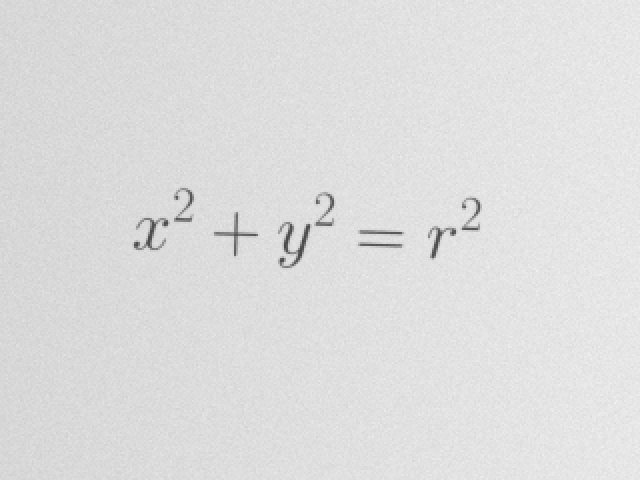
\includegraphics[width=0.47\linewidth]{img/fake_T26.png}\hfill
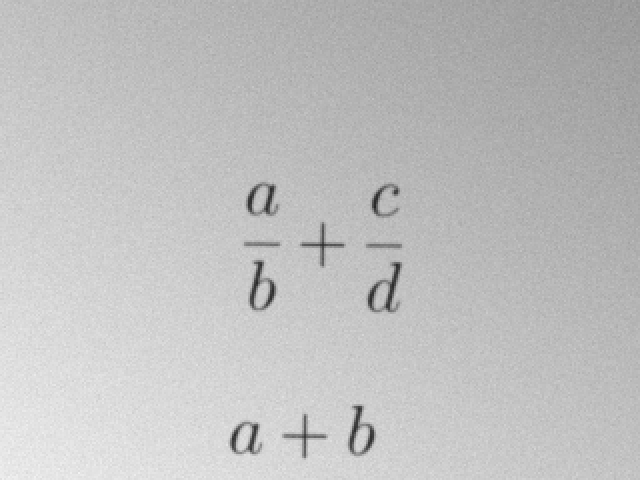
\includegraphics[width=0.47\linewidth]{img/fake_T47.png}
\caption{Two of the simulated photographs, \file{T26.png} and \file{T47.png}, shown enlarged.
A real frame from the board has the same size and a similar quality. Part of a neighbouring
printed line is visible at the bottom of the second photograph, as it would be on a real page;
the pipeline reads the line nearest the centre.}
\label{fig:fake}
\end{figure}

\begin{iffail}
If the output ends with \emph{pdflatex failed}, MiKTeX is not working: repeat
Steps~\ref{st:newafterinstall} to~\ref{st:verifytools}. If it says that \emph{pdftoppm (poppler)
is needed}, Poppler is not found: see Section~\ref{sec:trouble}. If a dialog of MiKTeX asks for
permission to install a package, click \ui{Install}, and afterwards run the command of
Step~\ref{st:autoinstall} again so that the question is not asked in future.
\end{iffail}

\subsection{Training images}

\step{Generate the synthetic training set}\label{st:synth}
\begin{ps}
python -m model.make_synthetic
\end{ps}
A classifier learns from examples. This command produces them without a camera: it draws every
one of the 182 symbols in every suitable font found on the laptop, and passes each drawing
through the same simulated camera as before, some 400 times per class with different sizes,
tilts, stroke weights and lighting.
\begin{out}[What you should see (abridged; the lead's laptop, 23 November)]
glyph bank: 6090 drawings from 31 font files + 5 mathtext sets; fewest: [...]; missing: []
bank built in 63 s -> C:\ee105\camera-to-latex\data\synthetic\glyph_bank.pkl
64600 crops for 159 classes in 20 s -> C:\ee105\camera-to-latex\data\synthetic\train.npz
segmentation check - members often split into pieces (tune MERGE_* in config.py):
  parallel         kept whole in 33% of drawings
  ...
preview pages: C:\ee105\camera-to-latex\data\synthetic/preview_*.png
\end{out}
\checkpoint{A line reports about 64{,}600 crops for 159 classes, and the list after
\emph{missing:} is empty (\texttt{[]}). The number of font files depends on the fonts installed
on the laptop and will differ from 31; that is expected. The lines about symbols ``split into
pieces'' are a diagnostic, not an error.}

To see what the classifier will learn from, run \code|explorer data\synthetic| and open
\file{preview\_1.png}: each row shows several generated images of one class.

\subsection{The classifier}

\step{Prepare the laptop for a long computation}
Training takes 45 to 75 minutes of uninterrupted computation. Connect the charger. Then make
sure that the laptop does not go to sleep: open \menu{Settings}\then\menu{System}\then\menu{Power
\& battery} (Windows~11) or \menu{Settings}\then\menu{System}\then\menu{Power \& sleep}
(Windows~10) and set the time after which the device sleeps \emph{when plugged in} to
\emph{Never}. Note the previous value so that you can restore it afterwards. Do not close the
lid during training.
\checkpoint{The charger is connected and sleep is switched off.}

\step{Train the convolutional neural network}\label{st:train}
\begin{ps}
python -m model.train
\end{ps}
The command reads the synthetic images, keeps 5\,\% of them aside for checking, and adjusts the
149{,}311 numerical weights of the network so that its answers on the remaining images improve.
One pass through all images is called an \term{epoch}; at most 30 are run, and training stops
earlier when the accuracy on the images kept aside has not improved for five epochs.
\begin{out}[What you should see at the start]
synthetic C:\ee105\camera-to-latex\data\synthetic\train.npz: 64600 crops
real crops: 0 (0 held out for testing)
training on 61385 crops, 159 classes, backend keras
model: 149311 weights
Epoch 1/30
\end{out}
After each epoch, which takes between one and three minutes, a line of figures is printed. The
figure to watch is \texttt{val\_accuracy}, the share of the images kept aside that were
classified correctly; it should rise above 0.9 within the first few epochs. Any lines about
\emph{oneDNN} or \emph{GPU support} at the start are informational. When training has finished,
a summary in braces is printed:
\begin{out}[What you should see at the end (the lead's laptop, 23 November)]
Epoch 24/30
480/480 - 86s - 179ms/step - accuracy: 0.9787 - loss: 0.0643 - val_accuracy: 0.9816 - val_loss: 0.0583 - learning_rate: 1.5625e-05
{
 "name": "symbols_v1",
 "backend": "keras",
 "crop_size": 32,
 "window_scale": 1.5,
 "features": "pixels",
 "weights": 149311,
 "trained": "2026-11-23 14:43",
 "minutes": 47.3,
 "data": {
  "synthetic": 61385,
  "real": 0,
  "real_repeat": 5,
  "external": 0
 },
 "synthetic_val_accuracy": 0.9835147744945568
}
\end{out}
\checkpoint{The summary shows \texttt{"backend": "keras"} and a value of
\texttt{synthetic\_val\_accuracy} of about 0.98 (between 0.97 and 0.99). The classifier has been
saved as \file{models\bs symbols\_v1.keras}, with its description in
\file{models\bs symbols\_v1.json}.}

\begin{note}[If time is short: the fallback classifier]
The command \code|python -m model.train --backend sklearn| trains a simpler classifier in two to
three minutes. It needs no TensorFlow and is slightly less accurate (0.974 against 0.984 on the
images kept aside). The rest of the quick start works with either. When both have been
trained, the pipeline uses the neural network.
\end{note}

\begin{iffail}[If the laptop slept, or the window was closed, during training]
Nothing is damaged. Open a new PowerShell window (Step~\ref{st:openps}) and give the three
commands below, one after the other. The training starts again from the beginning.
\end{iffail}
\begin{ps}[After an interruption, command 1 of 3]
cd C:\ee105\camera-to-latex
\end{ps}
\begin{ps}[After an interruption, command 2 of 3]
.\.venv\Scripts\Activate.ps1
\end{ps}
\begin{ps}[After an interruption, command 3 of 3]
python -m model.train
\end{ps}

\subsection{Accuracy of the complete pipeline}

\step{Evaluate on the 80 simulated photographs}\label{st:eval}
\begin{ps}
python -m tools.eval_pipeline --images test_set\synthetic --split all
\end{ps}
For each photograph the command runs the whole pipeline, compares the resulting \LaTeX{} with
the correct answer, and checks that the result compiles. It prints one line per photograph,
beginning with \texttt{ok} for a line read exactly right and with \texttt{-{}-} otherwise, and
then a summary table.
\begin{out}[What you should see (the lead's laptop, 23 November; most lines omitted)]
-- T01 plain     expected Hello World                  got Hello \textbackslash{}\textbackslash{}ror]d
ok T06 plain     expected a+b=c                        got a+b=c
ok T26 scripts   expected x^{2}+y^{2}=r^{2}            got x^{2}+y^{2}=r^{2}
ok T47 fractions expected \frac{a}{b}+\frac{c}{d}      got \frac{a}{b}+\frac{c}{d}

category   lines   exact     TER  compiles  s/line
plain         38   71.1%    9.8%    100.0%    0.54
scripts       23   60.9%   12.8%    100.0%    0.62
fractions     12   83.3%    7.2%    100.0%    0.37
mixed          7   57.1%   29.5%    100.0%    0.73
all           80   68.8%   12.0%    100.0%    0.55

per-line results: C:\ee105\camera-to-latex\results\eval_all_20261123_1450.csv
\end{out}

The columns of the table have the following meanings.
\begin{itemize}
\item \textbf{exact} is the share of lines whose \LaTeX{} equals the expected \LaTeX{} after both
  have been written in a standard form, so that differences of spacing, optional braces and
  synonyms such as \code|\le| and \code|\leq| do not count as errors.
\item \textbf{TER}, the token error rate, measures how wrong the lines are on average. A
  \term{token} is one unit of \LaTeX{}: a command such as \code|\alpha|, a brace, or a single
  character. With $d$ the smallest number of token insertions, deletions and substitutions that
  turn the output into the expected line (the edit distance), and $n$ the number of tokens of
  the expected line,
  \[
    \mathrm{TER} = \frac{d(\text{output},\ \text{expected})}{n} ,
  \]
  so that one wrong token in a line of 20 tokens gives 5\,\%.
\item \textbf{compiles} is the share of output lines that \cmd{pdflatex} accepts.
\item \textbf{s/line} is the computing time per photograph, in seconds, without the compile
  check.
\end{itemize}

\checkpoint{The table is printed, the row \emph{all} shows 80 lines, and the column
\emph{compiles} shows 100\,\%. Your percentages need not equal the ones above, because each
laptop trains a slightly different classifier; an overall \emph{exact} value between about 60\,\%
and 80\,\% is in the expected range at this size of lettering.}

\rationale{The value of about 69\,\% is the project's present state, not a fault of your
installation. Most errors arise when thin strokes break apart or neighbouring letters touch in
so small a picture; the companion document describes the measures taken against this.}

\step{Produce the review document}\label{st:review}
\begin{ps}
python -m tools.review_results
\end{ps}
\begin{out}
review: C:\ee105\camera-to-latex\results\review_all_20261124_1012.pdf
\end{out}
The command writes a PDF in which each test line occupies one row: the photograph with the
boxes that the pipeline drew, the expected line as typeset mathematics, and the line that the
pipeline produced, in orange when it is wrong (Figure~\ref{fig:review}). Open the folder with
\begin{ps}
explorer results
\end{ps}
and double-click the newest file whose name begins with \file{review\_}. The variant
\code|python -m tools.review_results --only-wrong| lists the misread lines only.
\checkpoint{The PDF opens and shows 80 rows of photographs with results.}

\begin{figure}[H]
\centering
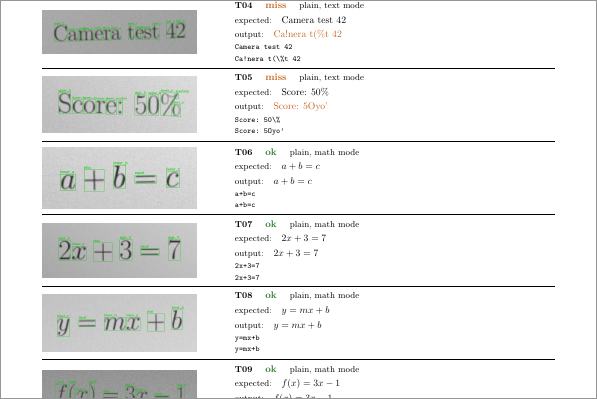
\includegraphics[width=0.86\linewidth]{img/review_page.png}
\caption{Part of a review document. Boxes in green mark symbols of which the classifier is
confident, boxes in red symbols of which it is not.}
\label{fig:review}
\end{figure}

\subsection{From one photograph to a PDF}

\step{Run the application on a stored photograph}\label{st:onephoto}
\begin{pswide}
python -m pipeline.main --new --image test_set\synthetic\T47.png --accept --pdf
\end{pswide}
This is the program that will later be used with the board, here given a stored photograph in
place of a live one. The option \code|--new| starts an empty document, \code|--accept| adds the
recognized line to it, and \code|--pdf| typesets the document and opens it.
\begin{out}
starting a new session
model symbols_v1 (keras, 159 classes)
test_set\synthetic\T47.png: [math] \frac{a}{b}+\frac{c}{d}  (612 ms)
accepted line 1: [math] \frac{a}{b}+\frac{c}{d}
PDF: C:\ee105\camera-to-latex\out\document.pdf
\end{out}
The time in parentheses will differ.
\checkpoint{A PDF opens in your PDF viewer and shows the sum of two fractions,
$\frac{a}{b}+\frac{c}{d}$, typeset as mathematics. If your classifier happened to misread a
symbol of this photograph the PDF shows that instead; the installation is correct either way,
because a PDF was produced.}

\subsection{Completion}

\step{Confirm the result and restore the power settings}
Tick the items of Table~\ref{tab:done}, restore the sleep setting that you changed before
training, and send the project lead a screenshot of the summary table of Step~\ref{st:eval}
(\key{Windows}+\key{Shift}+\key{S}).

\begin{table}[H]
\centering
\begin{tabular}{C{0.6cm}L{7.2cm}C{3.3cm}}
\toprule
 & \multicolumn{1}{c}{\hd{Result}} & \hd{Established in} \\
\midrule
\cbox & Four tools answer with a version number & Step~\ref{st:verifytools} \\
\cbox & The project is in \file{C:\bs ee105\bs camera-to-latex} & Step~\ref{st:gitclone} \\
\cbox & OpenCV 4 and TensorFlow 2 can be imported & Step~\ref{st:verifypy} \\
\cbox & All automatic tests pass & Step~\ref{st:pytest} \\
\cbox & 80 simulated photographs exist & Step~\ref{st:render} \\
\cbox & A classifier with about 98\,\% accuracy is stored in \file{models} & Step~\ref{st:train} \\
\cbox & The pipeline was scored on 80 lines, and every output compiled & Step~\ref{st:eval} \\
\cbox & One photograph became a PDF & Step~\ref{st:onephoto} \\
\bottomrule
\end{tabular}
\caption{Completion checklist for the set-up.}
\label{tab:done}
\end{table}

The quick start has created five folders inside the project: \file{data} (training images),
\file{models} (the classifier), \file{results} (evaluations), \file{out} (the PDF and its
sources) and \file{test\_set\bs synthetic} (the simulated photographs). Git is instructed, by
the file \file{.gitignore}, to leave all five on your laptop; they are never uploaded by
accident, and each can be regenerated with the commands of this section.
